\documentclass[aps,pre,reprint,twocolumn,nofootinbib,superscriptaddress]{revtex4-2}

\usepackage{amsmath,amssymb,amsthm}
\usepackage{graphicx}
\usepackage{bm}
\usepackage{xurl}
\usepackage{xcolor}
\usepackage{hyperref}

\hypersetup{
    pdfauthor={Taishi Namba},
    pdftitle={Can a learned score see the margin of the arrow of time?},
    pdfkeywords={coarse-graining, arrow of time, score-based diffusion models, denoising score matching, Fisher information, reverse-time SDE, Hamiltonian dynamics},
    hidelinks
}

\newtheorem{theorem}{Theorem}
\newtheorem{proposition}[theorem]{Proposition}
\newtheorem{lemma}[theorem]{Lemma}
\newtheorem{corollary}[theorem]{Corollary}
\newtheorem{observation}{Numerical result}
\theoremstyle{remark}
\newtheorem*{remark}{Remark}

\newcommand{\Sym}{\operatorname{Sym}}
\newcommand{\tr}{\operatorname{tr}}
\newcommand{\E}{\mathbb{E}}
\newcommand{\dv}{\operatorname{div}}
% Draft marker for items still to be filled in. Remove before release.
\newcommand{\pending}[1]{{\color{red}\textbf{[#1]}}}

\begin{document}

\title{Can a learned score see the margin of the arrow of time?}

\author{Taishi Namba}
\email{neginyan@gmail.com}
\affiliation{Independent Researcher, Atsugi, Kanagawa, Japan}

\date{\today}

\begin{abstract}
An observer who sees a Hamiltonian ensemble through a Gaussian window of width $\sigma(t) = \sigma_0 e^{rt}$ finds that the coarse-grained entropy grows if and only if $r$ exceeds a critical rate $R$ of the state, and $R$ stays below the largest strain rate $\kappa$ of the flow by a margin proportional to $\sigma$. The same forward process, a flow followed by a widening blur, defines a phase-space diffusion model. Here we ask whether a score learned from samples, as in a diffusion model, can see this margin. Two thresholds must be told apart. A forward or reverse-time stochastic differential equation that uses the physical flow as its drift exists only for $r \geq \kappa$, at every $\sigma$; the coarse-grained entropy, in contrast, keeps growing down to $r = R < \kappa$. We estimate $R$ in an integration-by-parts form in which each learned field appears once, so that its errors enter only linearly; we prove that errors orthogonal to the true fields leave this form exact while they bias the direct form, and find that for smooth random errors it is up to sixty times more accurate. Small networks trained by denoising score matching then read the margin $(\kappa - R)/\sigma$ to within $2.2\%$ at 36 points in a two-dimensional phase space (a pendulum, three kinds of states) and to within $1.4\%$ at 24 points in four dimensions (coupled pendulums). In four dimensions the learned margin agrees with the matrix formula for the resolution gap, including its finite-resolution correction, to within $2\%$. In the band $\kappa - c\sigma < r < \kappa$ the stochastic equation with the physical drift drifts away from the true law while the entropy, measured directly with nearest-neighbour estimators, keeps growing as predicted. The reverse equation fails exactly at $r = \kappa$, and the apparent knee slightly below $\kappa$ follows from the shape of the missing diffusion. All networks, results and checks are openly available.
\end{abstract}


\maketitle

\section{Introduction}
\label{sec:intro}

A Hamiltonian flow preserves the Gibbs entropy of every ensemble, yet an observer with a finite resolution sees an arrow of time. In a series of papers~\cite{namba2026arrow,namba2026gap,namba2026many} this was made quantitative for an observer who looks through a Gaussian window whose width grows as $\sigma(t) = \sigma_0 e^{rt}$. The coarse-grained entropy $S$ obeys
\begin{equation}
\frac{dS}{dt} = \sigma^2\,\tr F\,(r - R),
\label{eq:SC}
\end{equation}
with $F$ the Fisher matrix of the coarse-grained density and $R$ a critical rate of the state. For every Gaussian state $R \leq \kappa$, the largest symmetric strain rate of the flow~\cite{namba2026gap}, and the best state stays below $\kappa$ by a margin proportional to $\sigma$, the \emph{resolution gap}~\cite{namba2026gap}. In many degrees of freedom the gap is given by a matrix formula $\Gamma\sigma$, to which the best Gaussian state was found to come within a correction of order $\sigma^2$~\cite{namba2026many}.

The forward process behind Eq.~\eqref{eq:SC}, a deterministic flow followed by a widening Gaussian blur, is also the forward process of a phase-space diffusion model~\cite{dockhorn2022,namba2026threshold}. Diffusion models learn the score $\nabla\log p_t$ of the blurred density from samples and run the process backwards to generate~\cite{song2021,ho2020}. This suggests a question that connects the two fields. \emph{Can a score learned from samples see the margin of the arrow of time?} If it can, the margin becomes a measurable property of trained generative models, and the resolution gap of Refs.~\cite{namba2026gap,namba2026many} becomes testable with the tools of machine learning.

Answering the question requires separating two thresholds that are easily confused.
\begin{enumerate}
\item[(I)] A stochastic differential equation (SDE) with the physical flow as its drift and the widening blur as its noise exists only if the required diffusion matrix is positive semidefinite everywhere. This happens if and only if $r \geq \kappa$, at every $\sigma$ (Proposition~\ref{prop:sde}). Below $\kappa$ the noise would have to remove width along the stretching direction.
\item[(II)] The coarse-grained entropy grows if and only if $r > R$ (Eq.~\eqref{eq:SC}), and $R < \kappa$ by a margin proportional to $\sigma$.
\end{enumerate}
Between them lies a band $R < r < \kappa$ in which the arrow of time is present although no SDE with the physical drift can produce the blur. This article shows that a learned score sees both thresholds and the band between them. Our results are the following.
\begin{enumerate}
\item The critical rate can be estimated from learned fields in an integration-by-parts (divergence) form in which each learned field appears once, so that its errors enter only linearly. Errors orthogonal to the true fields leave this form exact but bias the direct form by the square of the score error (Proposition~\ref{prop:linear}). For smooth random errors the divergence form is 5 to 60 times more accurate, and in no case tested less accurate (Sec.~\ref{sec:estimators}).
\item Small networks trained by denoising score matching read the margin $(\kappa - R)/\sigma$ to within $2.2\%$ at 36 points of a pendulum (Sec.~\ref{sec:twodim}). In four dimensions (two coupled pendulums) they read it to within $1.4\%$ at 24 points, and agree with the formula of Ref.~\cite{namba2026many}, including its finite-resolution correction, to within $2\%$ (Sec.~\ref{sec:fourdim}).
\item In the band, the SDE with the physical drift departs from the true law while the entropy, measured directly with nearest-neighbour estimators, keeps growing as predicted. The reverse SDE fails exactly at $r = \kappa$ for every $\sigma$, in two and four dimensions, with exact and with learned scores. The apparent knee slightly below $\kappa$ is predicted by the shape of the missing diffusion (Sec.~\ref{sec:band}).
\end{enumerate}
Throughout, we separate what is proved from what is observed numerically, and we report the cases in which the learned score did not reach the required accuracy.

\section{Setting: one forward process, two thresholds}
\label{sec:setting}

\subsection{Forward process and entropy}

Let $\dot x = f(x)$ be a Hamiltonian flow on $\mathbb{R}^{2n}$ with flow map $\Phi_t$, and let $X_0$ have density $\rho_0$. The observer sees
\begin{equation}
Y_t = \Phi_t(X_0) + \sigma(t) Z, \qquad \sigma(t) = \sigma_0 e^{rt},
\label{eq:forward}
\end{equation}
with $Z$ standard normal and independent of $X_0$. The density of $Y_t$ is $p_t = \rho_t * N(0,\sigma^2 I)$, with $\rho_t$ the density of $X_t = \Phi_t(X_0)$. We write
\begin{equation}
s = \nabla \log p_t, \qquad m(y,t) = \E[f(X_t) \mid Y_t = y]
\end{equation}
for the score and for the conditional velocity, and $\E$ for the expectation over $Y_t \sim p_t$. Phase-space points are $x = (q, p)$; the letter $p$ also denotes the density $p_t$, and the meaning is always clear from the context.

\begin{proposition}[Fokker--Planck equation of the forward process]
\label{prop:fp}
For any smooth flow and any $\rho_0$ with finite second moments,
\begin{equation}
\partial_t p = -\dv(m\,p) + r\sigma^2 \Delta p .
\label{eq:fp}
\end{equation}
\end{proposition}
The proof (Appendix~\ref{app:fp}) combines the Liouville equation for $\rho_t$ with the heat equation in the variance $\sigma^2$, which grows at the rate $2r\sigma^2$. In the language of diffusion models~\cite{song2021}, the forward process has the marginals of a process with drift $m$ and diffusion coefficient $D = r\sigma^2$, that is, $g(t)^2 = d\sigma^2/dt = 2r\sigma^2$. Equation~\eqref{eq:fp} is exact; it requires no expansion in $\sigma$. Multiplying it by $-(1+\log p)$ and integrating by parts gives the entropy rate of $S = -\E[\log p_t]$,
\begin{gather}
\frac{dS}{dt} = r\sigma^2 \tr F + \Sigma, \label{eq:Sdot}\\
\tr F = \E|s|^2, \qquad \Sigma = -\E[s\cdot m], \nonumber
\end{gather}
which is Eq.~\eqref{eq:SC} with the critical rate
\begin{equation}
R = -\frac{\Sigma}{\sigma^2 \tr F} = \frac{\E[s\cdot m]}{\sigma^2\,\E|s|^2}.
\label{eq:R}
\end{equation}
The entropy grows if and only if $r > R$. This is threshold (II).

\subsection{The resolution gap}

Let $\lambda(x)$ be the largest eigenvalue of $\Sym Df(x)$ and $\kappa = \sup_x \lambda(x)$, the largest symmetric strain rate. For every Gaussian state $R \leq \kappa$~\cite{namba2026gap}, and in one degree of freedom the best Gaussian state has $(\kappa - R)/\sigma \to 2\sqrt{2\beta\kappa}$ as $\sigma\to 0$, where $\beta$ measures how fast $\lambda$ falls off around its maximum~\cite{namba2026gap}. For the pendulum, $H = p^2/2 - \cos q$, one has $\kappa = 1$ at the top $q = \pi$ and the limit is $1$. For $n$ degrees of freedom and $H = |p|^2/2 + V(q)$, the limit is bounded above by
\begin{equation}
\Gamma = 2\tr\big[(B^{1/2} C B^{1/2})^{1/2}\big],
\label{eq:Gamma}
\end{equation}
where $B$ is minus one half of the configuration-space Hessian of $\lambda$ at its maximum and $C = \operatorname{diag}(2\kappa, \kappa, \dots, \kappa)$; the optimum found numerically equals $\Gamma$, with a finite-resolution correction $(\kappa - R^*)/\sigma = \Gamma - c_1\sigma + O(\sigma^2)$~\cite{namba2026many}. We use two coupled pendulums,
\begin{equation}
V(q_1, q_2) = -\cos q_1 - \cos q_2 - \varepsilon \cos(q_1 - q_2),
\label{eq:coupled}
\end{equation}
with $\varepsilon = 0.1$ and $0.3$. Table~\ref{tab:systems} collects the constants. The quantity we want a learned score to see is the \emph{margin} $(\kappa - R)/\sigma$, which is of order one, while $\kappa - R$ itself is of order $\sigma$.

\begin{table}[t]
\caption{Systems used in this article. $\kappa$: largest symmetric strain rate; $\Gamma$: leading coefficient of the gap, Eq.~\eqref{eq:Gamma}; $c_1$: finite-resolution slope of the best Gaussian state, both from Ref.~\cite{namba2026many}.}
\label{tab:systems}
\begin{ruledtabular}
\begin{tabular}{lcccc}
system & dim. & $\kappa$ & $\Gamma$ & $c_1$ \\
\hline
pendulum & 2 & $1$ & $1$ & $7/8$ \\
coupled, $\varepsilon\!=\!0.1$ & 4 & $1.0525$ & $1.4025$ & $1.70$ \\
coupled, $\varepsilon\!=\!0.3$ & 4 & $1.1720$ & $1.8475$ & $2.38$ \\
\end{tabular}
\end{ruledtabular}
\end{table}

\subsection{A stochastic equation with the physical drift}

A diffusion model built on Eq.~\eqref{eq:forward} would like to write the forward process as a stochastic differential equation whose drift is the physical flow,
\begin{equation}
dY = \big(f(Y) + b(Y)\big)\,dt + G(Y)^{1/2}\, dW,
\label{eq:sde}
\end{equation}
so that the dynamics is known and only the score has to be learned. Matching the Fokker--Planck operator of Eq.~\eqref{eq:sde} to Eq.~\eqref{eq:fp}, with $m$ expanded in $\sigma$ around $y$, fixes the diffusion matrix and the drift correction (Appendix~\ref{app:sde}):
\begin{equation}
G = 2\sigma^2\big(rI - \Sym Df\big), \qquad b = \Big(0, \tfrac{\sigma^2}{2}\nabla_q \Delta_q V\Big).
\label{eq:G}
\end{equation}
For linear flows Eq.~\eqref{eq:sde} reproduces the law of $Y_t$ exactly; for nonlinear flows a remainder of third order in the expansion is left, of relative size $\sigma|\nabla^3 V|$ (for the pendulum, $\sigma|\sin q|$, which vanishes at the top). A diffusion matrix must be positive semidefinite.

\begin{proposition}[threshold (I)]
\label{prop:sde}
$G(y) \succeq 0$ for every $y$ if and only if $r \geq \kappa$. The condition does not depend on $\sigma$.
\end{proposition}
\begin{proof}
$G(y) \succeq 0$ if and only if $r \geq \lambda(y)$, and $\sup_y \lambda(y) = \kappa$. The factor $2\sigma^2 > 0$ does not change the sign.
\end{proof}
For a state that reaches the point of maximal strain, $r < \kappa$ means that the noise would have to \emph{remove} width there, along the stretching direction, faster than the flow adds it. No Brownian noise can do that. This is the threshold of Ref.~\cite{namba2026threshold}, stated here for the forward process~\eqref{eq:forward}. The same matrix enters the reverse-time equation~\cite{anderson1982,song2021}, whose drift is $f + b - \dv G - G s$ and whose noise is again $G^{1/2}$. By contrast, the probability-flow equation $\dot y = m - r\sigma^2 s$ follows from Eq.~\eqref{eq:fp} without any condition on $r$.

\subsection{The band}

Threshold (I) sits at $\kappa$ for every $\sigma$; threshold (II) sits at $R$, which for every Gaussian state is at most $\kappa$ and for the best one is about $\Gamma\sigma$ below it. In the band
\begin{equation}
R < r < \kappa
\label{eq:band}
\end{equation}
the coarse-grained entropy grows, but no stochastic equation with the physical drift produces the blur. The arrow of time seen by the observer is therefore not the arrow of a noisy physical dynamics: it is present where such a dynamics does not exist. The width of the band is the margin times $\sigma$, and reading it from data is the subject of the rest of this article.

\section{Estimating the critical rate from learned fields}
\label{sec:estimators}

A diffusion model provides a learned score $s_\theta \approx s$, and a second output can be trained to give $m_\theta \approx m$ by regressing $f(X_t)$ on $Y_t$. The question is how to combine them into $R$. Write $s_\theta = s + \delta s$, $m_\theta = m + \delta m$, and let $\eta_s = (\E|\delta s|^2/\E|s|^2)^{1/2}$ and $\eta_m$ be the relative $L^2(p_t)$ errors.

\subsection{Two forms}

The \emph{plain form} inserts the learned fields into Eq.~\eqref{eq:R},
\begin{equation}
R_{\rm plain} = \frac{\E[s_\theta\cdot m_\theta]}{\sigma^2\,\E|s_\theta|^2}.
\label{eq:Rplain}
\end{equation}
The \emph{divergence form} first integrates by parts, $\E[s\cdot m] = -\E[\dv m]$ and $\E|s|^2 = -\E[\dv s]$, and then inserts the learned fields,
\begin{equation}
R_{\rm div} = \frac{\E[\dv m_\theta]}{\sigma^2\,\E[\dv s_\theta]} .
\label{eq:Rdiv}
\end{equation}
Both are evaluated with samples of $Y_t$, which a diffusion model has by construction: data plus noise. The divergences are the traces of the Jacobians of the network outputs with respect to $y$, computed exactly through the network.

\begin{proposition}[errors enter the divergence form linearly]
\label{prop:linear}
Let $\delta s$ and $\delta m$ be differentiable fields with $p\,\delta s$ and $p\,\delta m$ vanishing at infinity. Then
\begin{align}
\E[\dv s_\theta] &= -\E|s|^2 - \E[s\cdot\delta s], \nonumber\\
\E[\dv m_\theta] &= -\E[s\cdot m] - \E[s\cdot\delta m],
\label{eq:linear}
\end{align}
whereas
\begin{align}
\E|s_\theta|^2 &= \E|s|^2 + 2\E[s\cdot\delta s] + \eta_s^2\,\E|s|^2, \nonumber\\
\E[s_\theta\cdot m_\theta] &= \E[s\cdot m] + \E[s\cdot\delta m] + \E[\delta s\cdot m] + \E[\delta s\cdot\delta m].
\label{eq:quadratic}
\end{align}
Consequently:
\begin{enumerate}
\item[(a)] for a scale error $s_\theta = (1+\eta)s$, $m_\theta = m$, both forms give $R/(1+\eta)$;
\item[(b)] for errors orthogonal to the true fields and to each other, $\E[s\cdot\delta s] = \E[s\cdot\delta m] = \E[\delta s\cdot m] = \E[\delta s\cdot\delta m] = 0$, the divergence form is exact, $R_{\rm div} = R$, while $R_{\rm plain} = R/(1+\eta_s^2)$.
\end{enumerate}
\end{proposition}
\begin{proof}
$\E[\dv u] = \int p\,\dv u = -\int \nabla p\cdot u = -\E[s\cdot u]$ for any field $u$ with $p u \to 0$; apply it to $u = s + \delta s$ and $u = m + \delta m$. Equation~\eqref{eq:quadratic} is the expansion of the products. For (a), $R_{\rm div} = \E[s\cdot m]/(\sigma^2(1+\eta)\E|s|^2)$ and $R_{\rm plain} = (1+\eta)\E[s\cdot m]/(\sigma^2(1+\eta)^2\E|s|^2)$. For (b), insert the vanishing terms into Eqs.~\eqref{eq:linear} and~\eqref{eq:quadratic}.
\end{proof}

The identities hold for learned fields because the expectation is taken under the \emph{true} law $p_t$, not under the law the network represents. In the divergence form a learned field appears once, and its error enters only through its projection on the true score. In the plain form the score error enters also through its square, $\eta_s^2\E|s|^2$, which is positive and cannot cancel, through the cross term $\E[\delta s\cdot\delta m]$, and through its projection $\E[\delta s\cdot m]$ on $m$ rather than on $s$. An error that oscillates on the scale $\sigma$ is nearly orthogonal to the smooth true fields, which is the situation of part (b): its linear terms largely cancel and only the extra terms of the plain form survive. Proposition~\ref{prop:linear} does not order the two forms for every error; with errors chosen so that the extra terms of the plain form cancel its linear terms, the plain form can come out closer. How the two forms compare for realistic errors is therefore a numerical question, answered next.

\subsection{Required accuracy}

Before training any network, we fixed the accuracy needed by adding artificial errors to the exact fields (Sec.~\ref{sec:learning} describes the exact fields). Three kinds were used: a smooth random field with correlation length $\sigma$ (twenty realizations; we report the 95th percentile of $|\Delta R|$), a scale error $(1+\eta)s$, and, in two dimensions, the exact score of a slightly wider blur. Figure~\ref{fig:required} shows the error of $R$ relative to the margin. For the scale error the two forms coincide, as Proposition~\ref{prop:linear}(a) states. For smooth random errors, as part (b) suggests, the divergence form is 5 to 16 times more accurate in two dimensions and 11 to 60 times in four dimensions, and in no case we tested is it less accurate. Table~\ref{tab:required} lists the largest $\eta$ that keeps $|\Delta R|$ below $10\%$ and $50\%$ of the margin for every kind of error. It is set by the scale error in four dimensions and therefore is the same for both forms there.

\begin{figure*}[t]
\centering
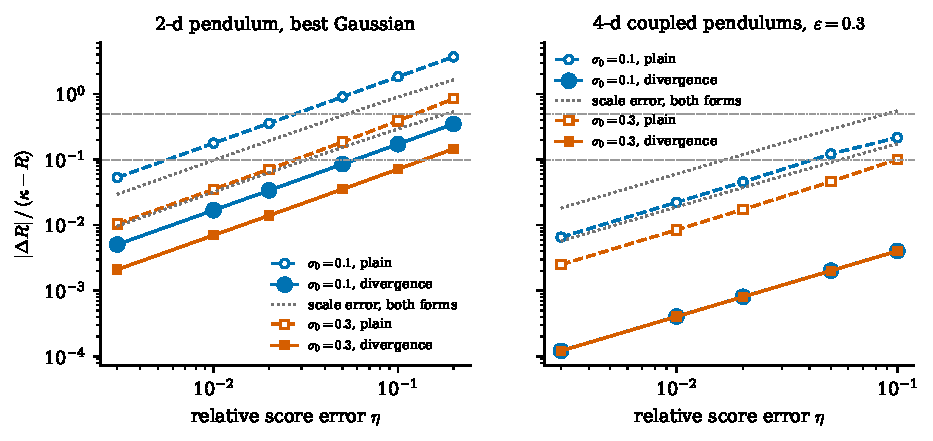
\includegraphics[width=0.85\textwidth]{figures/fig1_required_accuracy.pdf}
\caption{Error of the critical rate, relative to the margin $\kappa - R$, for a smooth random error of relative size $\eta$ in the score (95th percentile over twenty realizations, correlation length $\sigma$). Open symbols, dashed: plain form, Eq.~\eqref{eq:Rplain}. Filled symbols, solid: divergence form, Eq.~\eqref{eq:Rdiv}. Dotted: a scale error $(1+\eta)s$, for which both forms give $R/(1+\eta)$ exactly. Horizontal lines: $10\%$ and $50\%$ of the margin. Left: pendulum, best Gaussian state. Right: coupled pendulums, $\varepsilon = 0.3$, $W = 3$ state (Sec.~\ref{sec:fourdim}).}
\label{fig:required}
\end{figure*}

\begin{table}[t]
\caption{Required accuracy: the largest relative error $\eta$ (from the scanned values $0.003$, $0.01$, $0.02$, $0.05$, $0.1$, $0.2$) for which $|\Delta R|$ stays below $10\%$ / $50\%$ of the margin for every kind of error, at $t = 0$. Divergence form. ``$<$'': even $\eta = 0.003$ exceeds the criterion.}
\label{tab:required}
\begin{ruledtabular}
\begin{tabular}{llcc}
state & $\sigma_0$ & score & $m$ \\
\hline
pend., Gaussian & $0.3$ & $0.02$ / $0.1$ & $0.02$ / $0.1$ \\
 & $0.1$ & $0.01$ / $0.02$ & $0.003$ / $0.02$ \\
 & $0.03$ & $<$ / $0.01$ & $<$ / $0.003$ \\
pend., fan & $0.3$ & $0.02$ / $0.1$ & $0.02$ / $0.1$ \\
 & $0.1$ & $0.003$ / $0.02$ & $0.003$ / $0.02$ \\
coupled, $\varepsilon\!=\!0.1$ & $0.3$ & $0.02$ / $0.1$ & $0.02$ / $0.1$ \\
 & $0.1$ & $0.01$ / $0.05$ & $0.01$ / $0.05$ \\
coupled, $\varepsilon\!=\!0.3$ & $0.3$ & $0.05$ / $0.1$ & $0.05$ / $0.1$ \\
 & $0.1$ & $0.01$ / $0.05$ & $0.01$ / $0.05$ \\
\end{tabular}
\end{ruledtabular}
\end{table}

The table sets the target for learning: relative errors of about $1\%$ at $\sigma_0 = 0.1$ and a few percent at $\sigma_0 = 0.3$. At $\sigma_0 = 0.03$ the target is below $0.3\%$, which our networks did not reach (Sec.~\ref{sec:twodim}).

\section{Learning and exact references}
\label{sec:learning}

\emph{States.} In two dimensions we use three initial states near the top of the pendulum, each a Gaussian mixture of finite width: the best single Gaussian state at the given $\sigma_0$, a thin tilted segment through the top whose critical rate is the largest among Gaussian states~\cite{namba2026gap}; a continuous \emph{fan} of twenty segments, the best mixture found in the study of Ref.~\cite{namba2026gap}; and a \emph{needle}, a mixture of sixteen thin components found by adversarial search to have the smallest margin of all states tried (numerical study accompanying Ref.~\cite{namba2026many}). In four dimensions we use the best Gaussian state at the given $\sigma_0$ with all principal standard deviations at most $W = 3$; without this limit the optimum stretches far along the free momentum directions~\cite{namba2026many}, and its margin differs from that of the $W = 3$ state by $0.7\%$ at $\sigma_0 = 0.1$ and by $1.5$--$4.5\%$ at $\sigma_0 = 0.3$. The states are evolved for $0 \leq t \leq 0.5$ at $r = 1$ (two dimensions) or $r = \kappa$ (four dimensions); over this time the state leaves the top and the margin grows.

\emph{Networks.} Each network is a multilayer perceptron with three hidden layers of 128 units, SiLU activations and two output heads: the noise $\epsilon$ (equivalently the score, $s = -\epsilon/\sigma$) and $m$. Inputs are $(y, t, \log\sigma)$, with $y$ shifted by the position of the top in four dimensions. Training is by denoising score matching~\cite{vincent2011,hyvarinen2005} for the score and by regression of $f(X_t)$ on $Y_t$ for $m$, with two weightings of the score loss (the $\epsilon$ loss and the score loss, $\lambda(\sigma) = \sigma^2$ and $1$~\cite{ho2020,song2021}); the difference between them enters the error band. One network serves all rates $r$: during training $\sigma = \sigma_0 e^{\varrho t}$ with $\varrho$ drawn uniformly from $[0.55, 1.35]$ (times $\kappa$ in four dimensions). We use Adam with batch size 1024, 300\,000 steps, learning rate $2\times10^{-3}$ with cosine decay, and an exponential moving average of the weights. Training data are $4\times10^5$ (two dimensions) or $2\times10^5$ (four dimensions) samples of $X_0$, carried by the exact flow. All networks are written in NumPy and trained on one CPU core in float32, at about 4~ms per step. Twenty-four networks were trained (15.2~MB of weights).

\emph{Estimators.} The margin $(\kappa - R)/\sigma$ is evaluated with the divergence form~\eqref{eq:Rdiv} on $2\times10^5$ (two dimensions) or $5\times10^4$ (four dimensions) samples of $Y_t$, with the same random numbers at all $t$. The reported learned margin is the mean over the two weightings. Its error band is the sum of three parts: the difference between the weightings, the difference between the divergence form and a variant in which $m$ is replaced by the second-order Tweedie expression in the learned score~\cite{efron2011}, and two standard errors.

\emph{Exact references.} The initial mixture is replaced by quadrature nodes (trapezoid nodes with spacing at most $\sigma/4$ along wide directions in two dimensions and $\sigma/1.2$ in four, Gauss--Hermite nodes across thin directions). The nodes are carried by the exact flow (fourth-order Runge--Kutta, step $0.005$), and $p_t$, $s$, $m$ and their gradients are kernel sums. Refining the nodes changes the two-dimensional values by less than $10^{-9}$ at $t = 0.5$. In four dimensions we use between $5\times10^5$ and $6\times10^6$ nodes and evaluate expectations on samples, with standard errors below $0.3\%$ of the margin.

\emph{Entropy measured directly.} To test Eq.~\eqref{eq:SC} without any score, we measure $S(t+0.1) - S(t)$ with the Kozachenko--Leonenko nearest-neighbour estimator~\cite{kozachenko1987} ($k = 4$; $2\times10^6$ points in two dimensions and $4\times10^6$ in four, three repetitions each), using the same $X_0$ and $Z$ at both ends of each interval.

\section{The margin read by a learned score: two dimensions}
\label{sec:twodim}

\begin{figure*}[t]
\centering
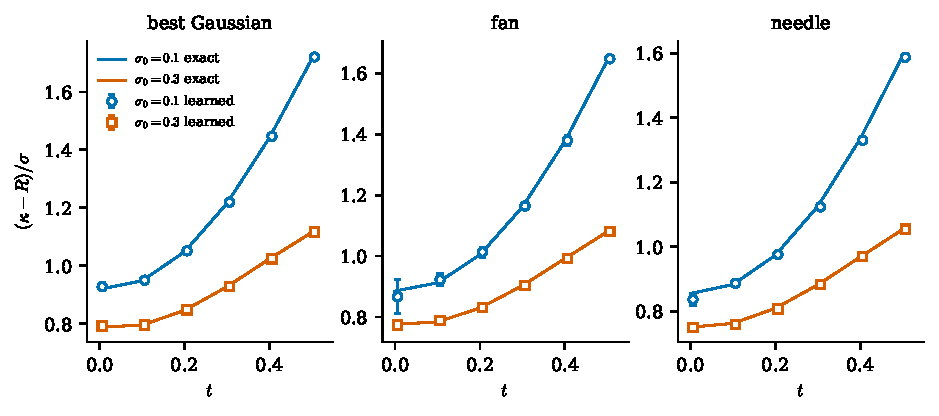
\includegraphics[width=0.9\textwidth]{figures/fig2_learned_2d.pdf}
\caption{Pendulum: the margin $(\kappa - R)/\sigma$ read from learned networks (symbols, with error band) against the exact value (lines), for $0 \leq t \leq 0.5$ at $r = 1$. Left to right: best Gaussian state, fan, needle. Circles: $\sigma_0 = 0.1$; squares: $\sigma_0 = 0.3$.}
\label{fig:learned2d}
\end{figure*}

\begin{observation}
\label{obs:2d}
For the three states and $\sigma_0 = 0.1$, $0.3$, the margin read from the learned networks with the divergence form agrees with the exact margin to within $2.15\%$ at all 36 points ($t = 0, 0.1, \dots, 0.5$). At 32 of them the difference lies inside the error band.
\end{observation}

Figure~\ref{fig:learned2d} shows the comparison. At $t = 0$ and $\sigma_0 = 0.1$ the distance $\kappa - R$ is only $8$--$9\%$ of $\kappa$, and the learned score resolves it with an error of at most about $2\%$ of itself, that is, $0.2\%$ of $R$. The two largest differences are at $t = 0$ and $\sigma_0 = 0.1$, for the fan ($-2.09\%$, inside a wide band) and for the needle ($-2.15\%$, outside its band). These are the sharpest states: their learned scores have $\eta_s = 0.013$ and $0.020$, above the $10\%$ target of Table~\ref{tab:required}, while for the best Gaussian state $\eta_s = 0.003$--$0.006$ and the differences stay below $1\%$. The other two points outside the band differ by $0.4$--$0.5\%$, where the band is narrow. As $t$ grows the state leaves the top, the margin grows, and the relative difference shrinks.

The form of the estimator is decisive. With the plain form~\eqref{eq:Rplain}, the same networks miss the margin of the best Gaussian state at $\sigma_0 = 0.1$, $t = 0$ by $14\%$; with the divergence form the miss is $1\%$.

\emph{The limit of our networks.} At $\sigma_0 = 0.03$ the required accuracy is $\eta < 0.003$ (Table~\ref{tab:required}). With batch size 16384 the learned score reached $\eta_s = 0.0018$--$0.0029$ for $0.1 \leq t \leq 0.5$, and the margin agreed with the exact one to within $0.7\%$ there, but at $t = 0$ it stayed at $\eta_s = 0.0036$, with a difference of $-2.1\%$. Increasing the batch size from 4096 to 16384 did not lower the error at $t = 0$, so gradient noise is no longer the limit there. We report $\sigma_0 = 0.03$ as a reference only and do not include it in the claims.

\section{Four dimensions and the formula for the gap}
\label{sec:fourdim}

\begin{figure*}[t]
\centering
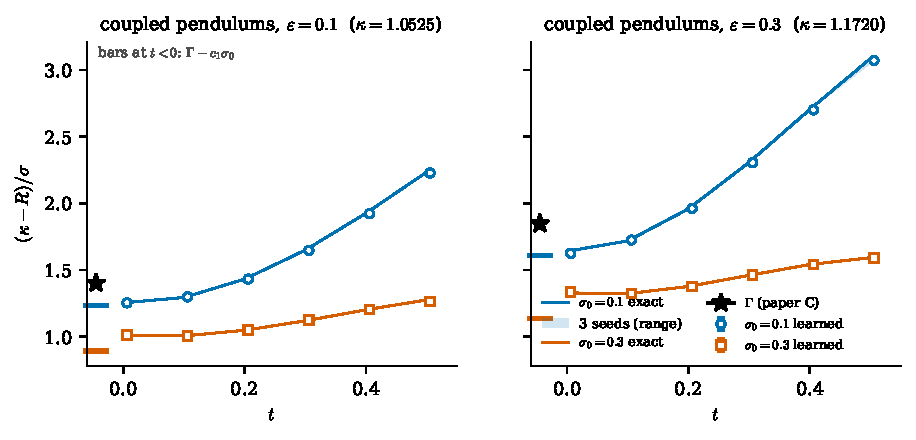
\includegraphics[width=0.9\textwidth]{figures/fig3_learned_4d.pdf}
\caption{Coupled pendulums, Eq.~\eqref{eq:coupled}: learned (symbols) and exact (lines) margins for $0 \leq t \leq 0.5$ at $r = \kappa$. Stars: $\Gamma$, the $\sigma \to 0$ limit of the best Gaussian state~\cite{namba2026many}; bars at $t<0$: $\Gamma - c_1\sigma_0$, the same with its finite-resolution correction. Shaded: range over three training seeds ($\varepsilon = 0.3$, $\sigma_0 = 0.1$).}
\label{fig:learned4d}
\end{figure*}

\begin{observation}
\label{obs:4d}
For $\varepsilon = 0.1$, $0.3$ and $\sigma_0 = 0.1$, $0.3$, the learned margin agrees with the exact margin to within $1.41\%$ at all 24 points, 21 of them inside the error band.
\end{observation}

The comparison is shown in Fig.~\ref{fig:learned4d}. The largest difference, $-1.41\%$, is again at $t = 0$, where the state is sharpest. Three networks trained with different seeds ($\varepsilon = 0.3$, $\sigma_0 = 0.1$) give margins whose standard deviation is $0.1$--$0.5\%$ and whose range is $0.2$--$1.0\%$ of the margin, comparable to the error band.

\begin{table}[t]
\caption{Four dimensions at $t = 0$: the margin of the $W = 3$ state, exact and learned, against the formula of Ref.~\cite{namba2026many}. $\Gamma - c_1\sigma_0$ includes the finite-resolution correction.}
\label{tab:fourdim}
\begin{ruledtabular}
\begin{tabular}{cccccc}
$\varepsilon$ & $\sigma_0$ & $\Gamma$ & $\Gamma - c_1\sigma_0$ & exact & learned \\
\hline
$0.1$ & $0.1$ & $1.4025$ & $1.2325$ & $1.2615$ & $1.2536$ \\
$0.3$ & $0.1$ & $1.8475$ & $1.6095$ & $1.6484$ & $1.6252$ \\
$0.1$ & $0.3$ & $1.4025$ & $0.8925$ & $1.0106$ & $1.0136$ \\
$0.3$ & $0.3$ & $1.8475$ & $1.1335$ & $1.3340$ & $1.3347$ \\
\end{tabular}
\end{ruledtabular}
\end{table}

\emph{Against the formula.} Table~\ref{tab:fourdim} compares the margin at $t = 0$ with the formula for the gap. At $\sigma_0 = 0.1$ the learned margin lies within $1.0$--$1.7\%$ of $\Gamma - c_1\sigma_0$, and the exact margin of the $W = 3$ state within $2.3$--$2.4\%$; both are $10$--$12\%$ below $\Gamma$ itself. The finite-resolution correction is therefore visible to the learned score. At $\sigma_0 = 0.3$ the linear correction overshoots: the margins lie $13$--$18\%$ above $\Gamma - c_1\sigma_0$, as expected when $c_1\sigma_0$ is no longer small compared with $\Gamma$. A network that never saw the formula thus reads a margin consistent with a matrix formula derived from the potential alone.

\emph{Entropy measured directly.} For $\varepsilon = 0.3$, $\sigma_0 = 0.1$, $r = \kappa$, we measured the entropy increase over five intervals of length $0.1$ with the nearest-neighbour estimator (Fig.~\ref{fig:entropy}, right). The prediction from the learned networks, Eq.~\eqref{eq:Sdot} integrated with the divergence form, agrees with the exact prediction to within $0.5\%$. The direct measurement brackets both: applied to the raw samples it is $0.5$--$6\%$ above, and applied after a global linear whitening it is $1$--$3\%$ below. The nearest-neighbour estimator is biased for a strongly anisotropic density with few neighbours per unit of the thin direction; whitening removes the anisotropy of the bulk but not that of the curved tails, which is why the two versions straddle the prediction. In two dimensions, where the bias is negligible, the measurement agrees with the exact entropy over all 30 intervals to within three standard errors, mostly within one (Fig.~\ref{fig:entropy}, left).

\begin{figure*}[t]
\centering
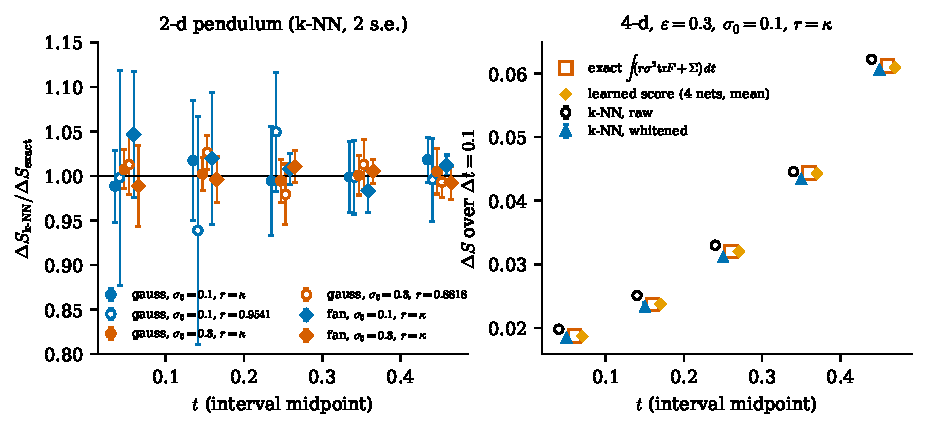
\includegraphics[width=0.9\textwidth]{figures/fig6_entropy.pdf}
\caption{Entropy increase measured directly with the Kozachenko--Leonenko estimator ($k = 4$), with no score. Left: pendulum, ratio of the measured to the exact increase over intervals of length $0.1$ (two standard errors), for $r = \kappa$ and for $r$ inside the band. Right: coupled pendulums, $\varepsilon = 0.3$, $\sigma_0 = 0.1$, $r = \kappa$: exact prediction $\int(r\sigma^2\tr F + \Sigma)\,dt$, the same from the learned networks (mean of four), and the nearest-neighbour measurement on raw and on whitened samples.}
\label{fig:entropy}
\end{figure*}

\section{The band between the two thresholds}
\label{sec:band}

\subsection{One state in the band}

Take the best Gaussian state of the pendulum at $\sigma_0 = 0.1$, whose critical rate is $R(0) = 0.9081$, and blur it at $r = 0.9541 = (\kappa + R(0))/2$, in the middle of the band~\eqref{eq:band}. Figure~\ref{fig:band} shows both thresholds for this one state.

\emph{(I)} The forward SDE~\eqref{eq:sde}, run with the positive part $G_+$ of $G$, departs from the true law: the error of the variance along the most stretching direction grows steadily to $6\%$ at $t = 1$. At $r = 1$ and $1.1$ it stays below $1\%$, the remainder of the expansion behind Eq.~\eqref{eq:G}.

\emph{(II)} The coarse-grained entropy, measured directly with the nearest-neighbour estimator, grows exactly as predicted: by $0.363$ over $0 \leq t \leq 1$, against $0.363$ predicted. Meanwhile $R(t)$ falls from $0.908$ to $0.272$ as the state leaves the top, so the entropy grows faster and faster.

In this state the arrow of time is present, and visible to a learned score, while the noisy physical dynamics that would produce the blur does not exist.

\begin{figure*}[t]
\centering
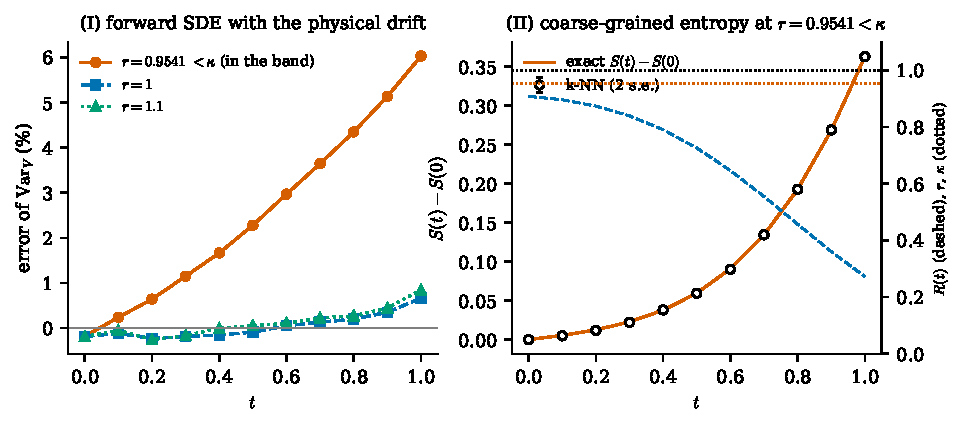
\includegraphics[width=0.9\textwidth]{figures/fig4_band.pdf}
\caption{One state in the band: pendulum, best Gaussian state, $\sigma_0 = 0.1$, $r = 0.9541$, between $R(0) = 0.9081$ and $\kappa = 1$. Left, threshold (I): relative error of the variance along the most stretching direction for the forward SDE with the physical drift and the clipped diffusion $G_+$; for comparison $r = 1$ and $1.1$. Right, threshold (II): entropy increase, exact (line) and measured with the nearest-neighbour estimator (circles, two standard errors); dashed, right axis: the critical rate $R(t)$; dotted: $r$ and $\kappa$.}
\label{fig:band}
\end{figure*}

\subsection{Where threshold (I) breaks}

To locate threshold (I) we scan $r/\kappa$ from $0.6$ to $1.3$ and measure, at the final time, the relative error of the variance along the most stretching direction (Fig.~\ref{fig:knee}). For the forward SDE we compare with the exact law. For the reverse direction we start from exact samples at the final time and run back both the reverse SDE with $G_+$ and the probability-flow equation, which needs no positive diffusion, with the same starting points; the difference isolates the effect of the missing diffusion. In four dimensions $\Sym Df$ depends on $q$, and $G$ is clipped pointwise: $G = U\operatorname{diag}(g)U^{\mathsf T}$, $G_+ = U\operatorname{diag}(\max(g,0))U^{\mathsf T}$.

\begin{observation}
\label{obs:knee}
In two and four dimensions, for $\sigma_0$ from $0.03$ to $0.3$ and with exact as well as learned scores, the error stays on a nearly flat plateau for $r \geq \kappa$ and grows as soon as $r < \kappa$. The learned score reproduces the curves of the exact score.
\end{observation}

The onset at $r = \kappa$ is exact: clipping happens only where $\lambda(q) > r$, which never occurs for $r \geq \kappa$ (Proposition~\ref{prop:sde}). Below $\kappa$ the error does not jump; it grows like a convex function of $\kappa - r$. If the curve is summarised by the zero of a straight line fitted through $r/\kappa = 0.8$, $0.9$ and $0.95$, this ``knee'' lies slightly below $\kappa$, further below for larger $\sigma_0$ and in four dimensions (Table~\ref{tab:knee}).

The shift has a simple origin. Clipping removes the diffusion $\sigma^2(\lambda - r)_+$ along the stretching direction, and only where the state has mass with $\lambda > r$. The total missing diffusion,
\begin{equation}
D(r) = \frac{1}{\sigma(T)^2}\int_0^T \E\big[\sigma(t)^2\,(\lambda(Y_t) - r)_+\big]\,dt ,
\label{eq:missing}
\end{equation}
vanishes for $r \geq \kappa$ and is convex below it, because a slightly smaller $r$ exposes only a small part of the state near the top. Applying the same straight-line rule to $D(r)$ gives a \emph{shape prediction} of the knee that uses no simulation of the SDE. It agrees with the measured knees to within $0.03$, and reproduces the trend with $\sigma_0$ and dimension (Table~\ref{tab:knee}). A wider state has more mass away from the top, so its exposure grows more slowly as $r$ decreases, and its knee lies further below $\kappa$. The knee is a property of the fit; the threshold is at $\kappa$.

\begin{table}[t]
\caption{Knee of threshold (I): zero of the straight line through $r/\kappa = 0.8$, $0.9$, $0.95$ of the difference between the reverse SDE and the probability-flow equation. Shape prediction: the same rule applied to the missing diffusion~\eqref{eq:missing}. Four dimensions: coupled pendulums, $\varepsilon = 0.3$.}
\label{tab:knee}
\begin{ruledtabular}
\begin{tabular}{ccccc}
dim. & $\sigma_0$ & exact score & learned score & shape \\
\hline
2 & $0.03$ & $1.005$ & $1.005$ & $0.987$ \\
2 & $0.1$ & $0.991$ & $0.990$ & $0.977$ \\
2 & $0.3$ & $0.972$ & $0.972$ & $0.965$ \\
4 & $0.1$ & $0.977$ & $0.960$ & $0.958$ \\
4 & $0.3$ & $0.978$ & $0.944$ & $0.951$ \\
\end{tabular}
\end{ruledtabular}
\end{table}

\begin{figure*}[t]
\centering
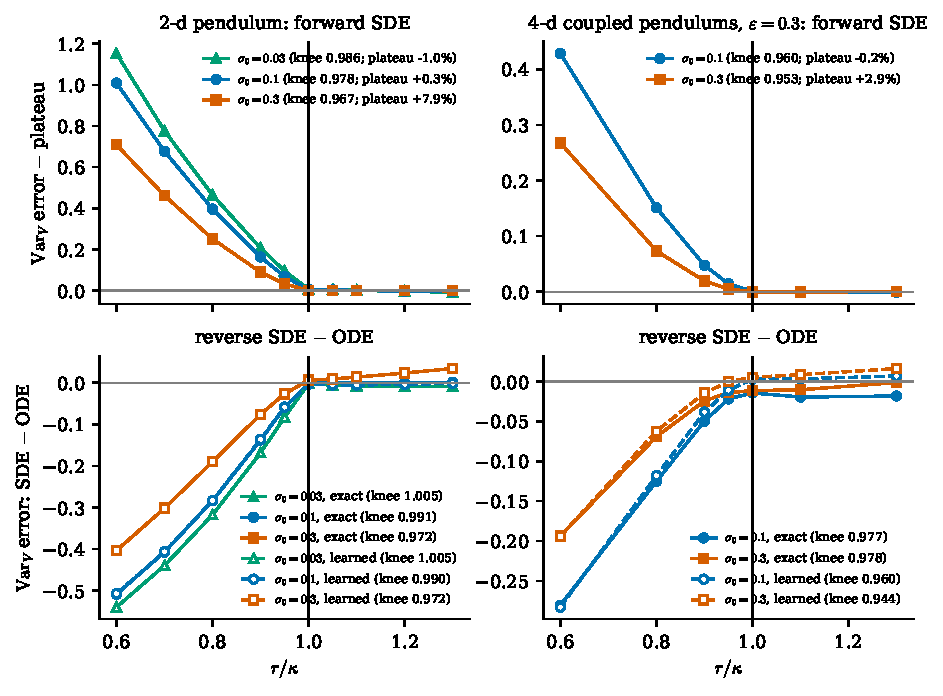
\includegraphics[width=0.9\textwidth]{figures/fig5_knee.pdf}
\caption{Threshold (I) as a function of $r/\kappa$. Top: forward SDE with the physical drift and $G_+$, relative error of the variance along the most stretching direction minus its plateau for $r \geq \kappa$. Bottom: reverse SDE minus probability-flow equation, with exact (filled) and learned (open) scores. Left: pendulum, $\sigma_0 = 0.03$, $0.1$, $0.3$. Right: coupled pendulums, $\varepsilon = 0.3$, $\sigma_0 = 0.1$, $0.3$. The vertical line is $r = \kappa$.}
\label{fig:knee}
\end{figure*}

In four dimensions the exact score is expensive, and the reverse runs used $2000$ paths with the exact score against $20\,000$ with the learned one; the difference between their knees ($0.017$--$0.034$) comes mostly from the small residual offset for $r \geq \kappa$, which differs between the two runs ($-0.011$ to $-0.020$ for the exact score, $+0.003$ to $+0.016$ for the learned one). Measured from the level at $r = \kappa$ instead of from zero, the four knees lie between $0.948$ and $0.964$, within $0.006$ of the shape prediction.

\section{Discussion}
\label{sec:discussion}

\emph{What was shown.} Proved: the forward process has the Fokker--Planck equation~\eqref{eq:fp} for any flow; a stochastic equation with the physical drift needs $r \geq \kappa$ at every $\sigma$ (Proposition~\ref{prop:sde}); and in the divergence form errors of learned fields enter the critical rate only linearly, so that errors orthogonal to the true fields leave it exact while the direct form is biased by the square of the score error (Proposition~\ref{prop:linear}). Observed: small networks trained by denoising score matching read the margin $(\kappa - R)/\sigma$ to within $2.2\%$ in two dimensions and $1.4\%$ in four; in four dimensions they agree with the formula for the gap, including its finite-resolution correction, to within $2\%$; in the band $R < r < \kappa$ the entropy grows as predicted while the stochastic equation with the physical drift fails; and the apparent knee below $\kappa$ is predicted by the shape of the missing diffusion.

\emph{Two arrows.} The two thresholds answer different questions. Threshold (II) asks whether the observer loses information: it depends on the state and on $\sigma$, and its margin is the resolution gap. Threshold (I) asks whether the loss can be produced by noise added to the physical dynamics: it depends only on the flow. The band between them shows that the coarse-grained arrow of time does not need a noisy dynamics behind it. For phase-space diffusion models, threshold (I) has a practical reading: a model that uses the physical flow as its drift must choose a noise rate of at least $\kappa$, the largest strain rate, whatever the noise level. Below it, the probability-flow equation remains available, because it requires no positive diffusion.

\emph{The estimator matters more than the network.} The same networks miss the margin by $14\%$ with the plain form and by $1\%$ with the divergence form. Any quantity that is a small difference of two large expectations of learned fields, as the margin is, should be computed in a form in which the learned fields appear once and are tested against the true law. The integration-by-parts identity of Proposition~\ref{prop:linear} achieves this for the entropy rate; it applies to any score-based model whose samples come from the true forward process.

\emph{Limitations.} The networks are small, written in NumPy and trained on one CPU core; we did not use a deep-learning framework. The phase spaces have two and four dimensions, where exact references can be computed by quadrature; in higher dimensions only the learned side and the direct entropy measurement would remain. In four dimensions the nearest-neighbour estimator is biased by a few percent, and only its raw and whitened versions together bracket the prediction. At $\sigma_0 = 0.03$ our networks did not reach the required accuracy at $t = 0$, and we make no claim there; a better allocation of training times near $t = 0$, or a larger network, may be needed. The expansion behind Eq.~\eqref{eq:G} leaves a third-order remainder, visible as a plateau of a few percent for $r \geq \kappa$ at $\sigma_0 = 0.3$.

\emph{Outlook.} The margin is a property of a state seen at a resolution, and the learned score made it measurable from samples alone. Two directions follow. One is molecular: the strain rates of a molecular force field and the noise schedules of generative models for molecular configurations are both defined in phase space, and the band~\eqref{eq:band} sets a lower limit on the noise rate of any such model that keeps the physical drift. The other is a uniform version of the gap, a bound $\kappa - R \geq c\sigma$ for all states and not only Gaussian ones, which the measurements here would allow to test on learned states.


\appendix
\section{Proofs}
\label{app:proofs}

\subsection{Proposition~\ref{prop:fp}}
\label{app:fp}

Let $\rho_t$ be the density of $X_t = \Phi_t(X_0)$; it obeys the Liouville equation $\partial_t\rho = -\dv(f\rho)$. Write $\phi_\sigma$ for the density of $N(0,\sigma^2 I)$, so that $p_t = \rho_t * \phi_{\sigma(t)}$. Since $\partial_{\sigma^2}\phi_\sigma = \tfrac12\Delta\phi_\sigma$ and $d\sigma^2/dt = 2r\sigma^2$,
\begin{align}
\partial_t p &= (\partial_t\rho) * \phi_\sigma + r\sigma^2\Delta p \nonumber\\
&= -\dv\big((f\rho)*\phi_\sigma\big) + r\sigma^2\Delta p .
\end{align}
Finally $(f\rho)*\phi_\sigma(y) = \int f(x)\rho(x)\phi_\sigma(y - x)\,dx = p(y)\,\E[f(X_t)\mid Y_t = y] = m\,p$. Finite second moments justify the exchange of derivatives and integrals. The entropy rate~\eqref{eq:Sdot} follows from $dS/dt = -\int (\partial_t p)\log p$ (the term $-\int\partial_t p$ vanishes), integration by parts, $\int\nabla p\cdot m = -\int p\,\dv m$, and $\int \nabla p \cdot \nabla \log p = \E|s|^2$.

\subsection{The diffusion matrix and the drift correction}
\label{app:sde}

By Tweedie's formula~\cite{efron2011}, $\E[X_t - y\mid y] = \sigma^2 s$ and $\E[(X_t - y)(X_t - y)^{\mathsf T}\mid y] = \sigma^2 I + \sigma^4(\nabla s + ss^{\mathsf T})$. Expanding $f(X_t)$ around $y$,
\begin{multline}
m\,p = f p + \sigma^2 Df\,\nabla p + \tfrac{\sigma^2}{2}(\Delta f)\,p \\
+ \tfrac{\sigma^4}{2}D^2 f : \nabla\nabla p + \dots ,
\label{eq:mexp}
\end{multline}
where $p(\nabla s + ss^{\mathsf T}) = \nabla\nabla p$ was used. The Fokker--Planck operator of Eq.~\eqref{eq:sde} is $-\dv((f+b)p) + \tfrac12\partial_i\partial_j(G_{ij}p)$. Split $Df = \Sym Df + A$ with $A$ antisymmetric. For a mechanical flow, $f = (\nabla_p H, -\nabla_q H)$ with $H = |p|^2/2 + V(q)$, one has $\dv f = 0$, hence $\partial_i (Df)_{ij} = 0$, $\partial_j (Df)_{ij} = \Delta f_i$, $\partial_i A_{ij} = -\tfrac12\Delta f_j$ and $\partial_j(\Sym Df)_{ij} = \tfrac12\Delta f_i$. With $G = 2\sigma^2(rI - \Sym Df)$,
\begin{multline}
\tfrac12\partial_i\partial_j(G_{ij}p) = r\sigma^2\Delta p - \sigma^2\partial_i\big((\Sym Df)_{ij}\partial_j p\big) \\
 - \tfrac{\sigma^2}{2}\dv\big((\Delta f)p\big),
\end{multline}
while the first three terms of Eq.~\eqref{eq:mexp} give
\begin{multline}
-\dv(mp) + r\sigma^2\Delta p = -\dv(fp) + r\sigma^2\Delta p \\
- \sigma^2\partial_i\big((\Sym Df)_{ij}\partial_j p\big) + \tfrac{\sigma^2}{2}(\Delta f)\cdot\nabla p \\
- \tfrac{\sigma^2}{2}\dv\big((\Delta f)p\big) ,
\end{multline}
using $\partial_i(A_{ij}\partial_j p) = (\partial_i A_{ij})\partial_j p$. The two agree if $-\dv(bp) - \tfrac{\sigma^2}{2}\dv((\Delta f)p) = \tfrac{\sigma^2}{2}(\Delta f)\cdot\nabla p - \tfrac{\sigma^2}{2}\dv((\Delta f)p)$, that is, since $\dv\Delta f = \Delta\dv f = 0$, if $b = -\tfrac{\sigma^2}{2}\Delta f = (0, \tfrac{\sigma^2}{2}\nabla_q\Delta_q V)$. This is Eq.~\eqref{eq:G}. For a linear flow $D^2 f = 0$, $b = 0$, and the expansion~\eqref{eq:mexp} terminates, so the SDE reproduces the law of $Y_t$ exactly. Otherwise the last term of Eq.~\eqref{eq:mexp} is a third-order (Kramers--Moyal) term; since $\nabla p \sim p/\sigma$ across a thin state, it is smaller than the diffusion term by a factor of order $\sigma|D^2 f|$. For the pendulum $b = (0, -\tfrac{\sigma^2}{2}\sin q)$ and the relative remainder is of order $\sigma|\sin q|$.

\section{Methods}
\label{app:methods}

\emph{Error of the learned fields.} $\eta_s$ and $\eta_m$ are the relative $L^2(p_t)$ errors against the exact fields, on the same samples as the margin. In two dimensions $\eta_s = 0.003$--$0.006$ for the best Gaussian state and $0.009$--$0.020$ for the fan and the needle, with $\eta_m = 0.001$--$0.010$; in four dimensions $\eta_s = 0.009$--$0.051$ and $\eta_m = 0.0006$--$0.008$, the larger values at $t = 0.5$ where the margin is largest.

\emph{Stochastic equations.} The forward SDE~\eqref{eq:sde} is integrated with the Euler--Maruyama scheme (step $0.005$) from exact samples of $Y_0$, with $2\times10^4$ to $5\times10^4$ paths. The reverse runs start from exact samples of $Y_T$ ($T = 1$ in two dimensions, $T = 0.5$ in four) and use step $0.005$ (two dimensions) or $0.01$ (four dimensions); the same noise is used for every $r$, and the reverse SDE and the probability-flow equation start from the same points. In four dimensions $\dv G_+$ is computed by central differences in $q$ (step $10^{-5}$), and $G_+^{1/2} = U\operatorname{diag}(\max(g,0)^{1/2})U^{\mathsf T}$. The measured quantity is the relative error of the variance along the most stretching direction at the top, compared with the exact law.

\emph{Knee.} A straight line is fitted through the points $r/\kappa = 0.8$, $0.9$, $0.95$ of the reverse SDE minus probability-flow difference, and its zero is the knee. The missing diffusion~\eqref{eq:missing} is evaluated on $2\times10^4$ samples of the exact law at each time.

\emph{Nearest-neighbour entropy.} The Kozachenko--Leonenko estimator~\cite{kozachenko1987} with $k = 4$ is applied to the same $X_0$ and $Z$ at the two ends of each interval, which cancels most of the sampling noise in the difference. In four dimensions the whitened version applies one fixed linear map, the whitening map of the covariance of $Y_0$, at all times; it changes the entropy by a known constant that cancels in the difference.

\emph{Verification.} Every number in this article is produced from stored results by one script, and a verification suite checks it against its source with a stated tolerance, using at most $20\%$ of each tolerance. The suite recomputes the learned margins from the stored network weights (agreement to $5\times10^{-8}$), recomputes the two-dimensional exact values, checks the clipping of $G$ in four dimensions, and, optionally, retrains networks from their seeds and compares the weights bit for bit. The suite has 29 checks; a further 39 checks of the analytical statements and of selected numbers were written separately from the study code. All pass.


\section*{Acknowledgments}
The author used AI assistants in this work: Google Gemini (\mbox{Gemini 3.8 Flash}), OpenAI ChatGPT (\mbox{GPT-5.6 Luna}) and Anthropic Claude (\mbox{claude-opus-5-5}). They were used for derivations, for writing and running the numerical study and its verification code, for independent cross-checking, and for drafting the text. The author conceived the research program and the question of this article, directed the work, decided what is claimed, and takes full responsibility for its content.

\section*{Data and Code Availability}
Scripts, trained network weights and results that reproduce every number and figure of this article, together with the verification suite, are openly available at \url{https://github.com/neginyan/learned-score-arrow-of-time}. The version used for this article is archived at Zenodo, \pending{DOI}.


\begin{thebibliography}{99}

\bibitem{namba2026arrow}
T.~Namba, \textit{Sharp criterion for the coarse-grained arrow of time in Hamiltonian dynamics}, preprint, version v1.2, Zenodo (2026), \href{https://doi.org/10.5281/zenodo.23258135}{doi:10.5281/zenodo.23258135}.

\bibitem{namba2026gap}
T.~Namba, \textit{A resolution gap for the coarse-grained arrow of time in nonlinear Hamiltonian flows}, preprint, version v1.1, Zenodo (2026), \href{https://doi.org/10.5281/zenodo.23320603}{doi:10.5281/zenodo.23320603}.

\bibitem{namba2026many}
T.~Namba, \textit{The resolution gap in many degrees of freedom}, preprint, version v1.0, Zenodo (2026), \href{https://doi.org/10.5281/zenodo.23371932}{doi:10.5281/zenodo.23371932}.

\bibitem{namba2026threshold}
T.~Namba, \textit{A stretching-rate threshold for phase-space diffusion models with isotropic marginal noise schedules}, preprint, Zenodo (2026), \href{https://doi.org/10.5281/zenodo.23181225}{doi:10.5281/zenodo.23181225}.

\bibitem{song2021}
Y.~Song, J.~Sohl-Dickstein, D.~P. Kingma, A.~Kumar, S.~Ermon, and B.~Poole, \textit{Score-based generative modeling through stochastic differential equations}, in \textit{International Conference on Learning Representations} (2021).

\bibitem{ho2020}
J.~Ho, A.~Jain, and P.~Abbeel, \textit{Denoising diffusion probabilistic models}, in \textit{Advances in Neural Information Processing Systems} \textbf{33}, 6840 (2020).

\bibitem{dockhorn2022}
T.~Dockhorn, A.~Vahdat, and K.~Kreis, \textit{Score-based generative modeling with critically-damped Langevin diffusion}, in \textit{International Conference on Learning Representations} (2022).

\bibitem{vincent2011}
P.~Vincent, \textit{A connection between score matching and denoising autoencoders}, Neural Comput. \textbf{23}, 1661 (2011).

\bibitem{hyvarinen2005}
A.~Hyv\"arinen, \textit{Estimation of non-normalized statistical models by score matching}, J. Mach. Learn. Res. \textbf{6}, 695 (2005).

\bibitem{anderson1982}
B.~D.~O. Anderson, \textit{Reverse-time diffusion equation models}, Stoch. Proc. Appl. \textbf{12}, 313 (1982).

\bibitem{efron2011}
B.~Efron, \textit{Tweedie's formula and selection bias}, J. Am. Stat. Assoc. \textbf{106}, 1602 (2011).

\bibitem{kozachenko1987}
L.~F. Kozachenko and N.~N. Leonenko, \textit{Sample estimate of the entropy of a random vector}, Probl. Inf. Transm. \textbf{23}, 95 (1987).

\end{thebibliography}


\end{document}
